\documentclass[a4paper,12pt]{article}
\usepackage{amsmath,amsfonts,amssymb} % Math packages
\usepackage{mathtools} % For defining floor and ceiling functions
\usepackage{amsthm}    % Theorems
\usepackage{bm} 	   % Bold math
\usepackage{bbm}	   % More bold math?
\usepackage{array}     % Better tables
\usepackage{chemfig}   % chemical figures
\usepackage{physics}   % derivatives and partials
\usepackage{float}     % Better positioning [H]
\usepackage{framed}    % Framed boxes
\usepackage{geometry}  % Required for adjusting page dimensions and margins
\usepackage{graphicx}  % Include images
\usepackage{multirow}  % multicolumn tables
\usepackage{pgfplots}  % Create plots in latex
\usepackage{siunitx}   % SI unit system
\usepackage{listings}  % Code environments
\usepackage[shortlabels]{enumitem} %lets us change the enumeration to (a), (b), ...
\usepackage{booktabs}  % Better looking horizontal rules
\usepackage{makecell}  % Pre-formatting of column heads
\usepackage{hyperref}  % Clickable links
\renewcommand{\arraystretch}{1.6}

% Theorems and definitions
\theoremstyle{definition}
\newtheorem*{definition}{Definition}
\pgfplotsset{width=10cm,compat=1.9}

% Graph drawings
\usetikzlibrary{shapes,arrows,positioning,} % Graph arrows
\usetikzlibrary{automata,positioning,fit,shapes.geometric,backgrounds} % Node grouping

% stats commands
\newcommand{\E}{\mathbb{E}}
\newcommand{\Var}{\mathbb{V}\mathrm{ar}}
\newcommand{\Cov}{\mathbb{C}\mathrm{ov}}
\newcommand{\Risk}{\mathcal{R}}

% common number sets
\newcommand{\N}{\mathbb{N}}
\newcommand{\R}{\mathbb{R}}
\newcommand{\Q}{\mathbb{Q}}
\newcommand{\Z}{\mathbb{Z}}
\newcommand{\C}{\mathbb{C}}

% Cs stuff
\newcommand{\bigO}{\mathcal{O}}

% Indicator function
\newcommand{\Ind}[1]{\mathbbm{1}_{\{#1\}}}

\DeclarePairedDelimiter\ceil{\lceil}{\rceil}
\DeclarePairedDelimiter\floor{\lfloor}{\rfloor}
\DeclarePairedDelimiter\angleb{\langle}{\rangle}

\geometry{
	paper=a4paper, % Paper size, change to letterpaper for US letter size
	top=2.5cm, % Top margin
	bottom=2.5cm, % Bottom margin
	left=2.5cm, % Left margin
	right=2.5cm, % Right margin
	headheight=14pt, % Header height
	footskip=1.5cm, % Space from the bottom margin to the baseline of the footer
	headsep=1.2cm, % Space from the top margin to the baseline of the header
}

\lstset{
	basicstyle=\ttfamily,
	mathescape,
	inputencoding=utf8,
	escapeinside={\%*}{*)},
	literate={á}{{\'a}}1 {ã}{{\~a}}1 {é}{{\'e}}1 {É}{{\'E}}1 {è}{{\`e}}1 {à}{{\`a}}1,
	numbers=left,
	breaklines=true
}

\let\tss\textsuperscript % superscript macro
\let\oldtextbf\textbf
\renewcommand{\textbf}[1]{\oldtextbf{\boldmath #1}}

\newtheorem{exercise}{Exercise}[section]

\begin{document}
\title{Deep Learning}
\author{David Zhao}
\date{Febrary 9, 2023}
\maketitle

\section{Preface}
This paper is a learning documentation adapted/copied from the book \href{https://d2l.ai/}{Dive into Deep learning}.
Coding implementations are omitted (for now).

\section{Preliminaries}
    \subsection*{AutoDifferentiation}

    \subsection*{Linear Algebra}
    \subsubsection*{Norms}
    Some of the most useful operators in linear algebra are norms. Informally, the norm of a vector tells us how big it is.
    Here, we are employing a notion of size that concerns the magnitude of a vector’s components (not its dimensionality).

    A norm is a function $||\cdot||$ that maps a vector to a scalar and satisfies the following three properties:
    \begin{enumerate}
        \item Given any vector $\mathbf{x}$, if we scale the vector by a scalar $\alpha \in \R$, its norm scales accordingly:
        \begin{equation*}
            \begin{aligned}
                ||\alpha\mathbf{x}|| = |\alpha|||\mathbf{x}||
            \end{aligned}
        \end{equation*}
        \item For any vectors $\mathbf{x}$ and $\mathbf{y}$, norms must satisfy the triangle inequality:
        \begin{equation*}
            \begin{aligned}
                ||\mathbf{x} + \mathbf{y}|| = ||\mathbf{x}|| + ||\mathbf{y}||
            \end{aligned}
        \end{equation*}
        \item The norm of a vector is nonnegative and vanishes if and only if the vector is zero: 
        \begin{equation*}
            \begin{aligned}
                ||\mathbf{x}|| > 0 \iff \mathbf{x} \neq 0
            \end{aligned}
        \end{equation*}
    \end{enumerate}
    For instance, the $l2$ norm measures the (Euclidean) length of a vector which we've all seen already in school when calculating the hypotenuse of a right triangle..
    Formally, we know it as
    \begin{equation*}
        \begin{aligned}
            ||\mathbf{x}||_2 = \sqrt{\sum_{i=1}^{n}\mathbf{x}_i^2}
        \end{aligned}
    \end{equation*}
    The $l1$ norm is also popular and the associated metric is called the Manhattan distance. By definition, the 
    norm sums the absolute values of a vector's elements:
    \begin{equation*}
        \begin{aligned}
            ||\mathbf{x}||_1 = \sum_{i=1}^{n}|\mathbf{x}_i|
        \end{aligned}
    \end{equation*}
    Both the $l1$ and $l2$ norms are special cases of the more general norms:
    \begin{equation}
        \begin{aligned}
            ||\mathbf{x}||_p = \left({\sum_{i=1}^{n}\mathbf{x}_i^p}\right)^{1/p}
        \end{aligned}
    \end{equation}
    \subsection*{Chain Rule}
    Let $y = f(\mathbf{u})$ such that $\forall i, \mathbf{u}_i = g_i(\mathbf{x})$ where $\mathbf{u} = (u_1, u_2, \ldots, u_m)$ and $\mathbf{x} = (x_1, x_2, \ldots, x_n)$. \\
    Then
    \begin{equation}
        \begin{aligned}
            \frac{\partial y}{\partial x_i} = \frac{\partial y}{\partial u_1}\frac{\partial u_1}{\partial x_i} + \ldots + \frac{\partial y}{\partial u_m}\frac{\partial u_m}{\partial x_i} 
        \end{aligned}
    \end{equation}

    \subsection*{Baye's Theorem}
    Given any event A and B such that $P(B) \neq 0$, 
    \begin{equation}
        \begin{aligned}
            P(A|B) = \frac{P(B|A)P(A)}{P(B)}
        \end{aligned}
    \end{equation}

    \subsection*{Expectations}

\section{Linear Neural Networks for Regression}
    We assume that the relationship between features $\mathbf{x}$ and target $y$ is approximately linear, i.e,
    \begin{equation}
        E[Y|X=\mathbf{x}] = x_1w_1 + \ldots + x_dw_d + b \\
    \end{equation}
    where $d$ is the \textit{feature dimensionality}, and $b$ is the \textit{bias}. As such,
    \begin{equation}
        \begin{aligned}
        \hat{y} &= \mathbf{w}^T\mathbf{x} + b
                &= \mathbf{Xw} + b
        \end{aligned}
    \end{equation}
    In essence, our goal is to find parameters $\mathbf{w}$ and $b$ such that our prediction error is 
    minimized for new data examples that are sampled from the same distribution X.
    \begin{figure}[h]
        \centering
        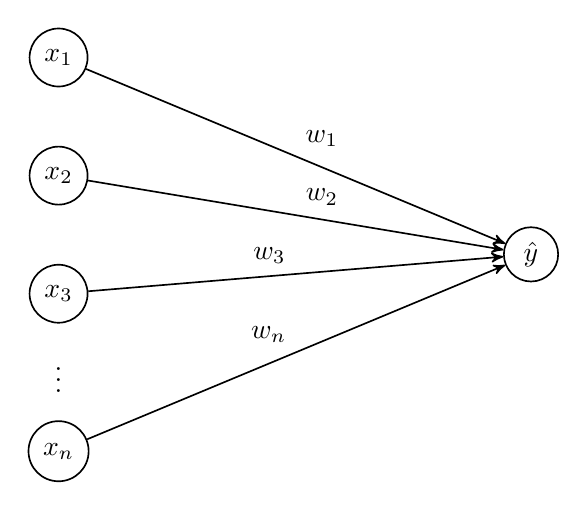
\begin{tikzpicture}[->, >=stealth', auto, semithick, node distance=3cm]
        \tikzstyle{every state}=[fill=white,draw=black,thick,text=black,scale=1]
        \node[draw, circle]    (x1) at (0,0)        {$x_1$};
        \node[draw, circle]    (x2) at (0,-1.5)     {$x_2$};
        \node[draw, circle]    (x3) at (0,-3)       {$x_3$};
        \node[draw, circle]    (xn) at (0,-5)       {$x_n$};
        \node[draw, circle]    (y) at (6,-2.5)      {$\hat{y}$};
        \begin{scope}[on background layer]
        \end{scope}
        \path
        (x1) edge[]	node{$w_1$}	(y)
        (x2) edge[]	node{$w_2$}	(y)
        (x3) edge[]	node{$w_3$}	(y)
        (x3) -- node[auto=false]{\vdots} (xn)
        (xn) edge[]	node{$w_n$}	(y);
        \end{tikzpicture}
        \caption{Linear Regression Model with feature dimensionality $n$}
    \end{figure}
    \subsection*{Loss Function}
    Naturally, our model requires an objective measure of how well or unwell it fits the training data.
    Loss functions fill in this role by quantifying the distance between the \textit{observed} and \textit{predicted}
    labels. The most commonly used loss function is the squared error.
    \begin{equation}
        l^{(i)}(\mathbf{w},b) = \frac{1}{2}(\hat{y}^{(i)}-\mathbf{y}^{(i)})^2
    \end{equation}
    Note that the presence of the constant coefficient $\frac{1}{2}$ is notationally convenient as it disappears when we
    take the derivative of the loss function. Also notice that large differences between estimates $\hat{y}^{(i)}$ 
    and targets $\mathbf{y}^{(i)}$ lead to larger contributions due to the function's quadratic form. In fact, while
    it does encourage our model to avoid sizeable errors, it also yields an excessive sensitivity to anomalous data.
    Finally, to evaluate our model's performance over entire the dataset of $n$ examples, we simply take the average of 
    the losses on the training set:
    \begin{equation}
        L^{(i)}(\mathbf{w},b) = \frac{1}{n}\sum_{i=1}^{n}\frac{1}{2}(\hat{y}^{(i)}-\mathbf{y}^{(i)})^2
    \end{equation}
    Hence, our goal is to find parameters $\mathbf{w}^*$ and $b^*$ such that 
    the total loss is minimized across all examples.

    \subsection*{Minibatch Stochastic Gradient Descent}
    \begin{equation*}
        \begin{aligned}
        (\mathbf{w},b) &\leftarrow (\mathbf{w},b) - \frac{\eta}{|\beta|}\sum_{i\in\beta_i}\frac{\partial}{\partial(\mathbf{w},b)}l^{(i)}(\mathbf{w},b) \\
        \mathbf{w}     &\leftarrow \mathbf{w} - \frac{\eta}{|\beta|}\sum_{i\in\beta_i}\frac{\partial}{\partial\mathbf{w}}l^{(i)}(\mathbf{w},b) = \mathbf{w}- \frac{\eta}{|\beta|}\sum_{i\in\beta_i}\mathbf{x}^{(i)}(\mathbf{w}^T\mathbf{x}^{(i)} + b - \mathbf{y}^{(i)}) \\
        b           &\leftarrow b - \frac{\eta}{|\beta|}\sum_{i\in\beta_i}\frac{\partial}{\partial b}l^{(i)}(\mathbf{w},b) = \mathbf{w}- \frac{\eta}{|\beta|}\sum_{i\in\beta_i}(\mathbf{w}^T\mathbf{x}^{(i)} + b - \mathbf{y}^{(i)})
        \end{aligned}
    \end{equation*}

    \subsection*{Normal Distribution and Squared Loss}
    So far we have given a fairly functional motivation of the squared loss objective: the optimal parameters return the conditional expectation 
    whenever the underlying pattern is truly linear, and the loss assigns outsize penalties for outliers. We can also provide a more formal motivation for the squared loss objective by making probabilistic assumptions about the distribution of noise.

    To begin, recall that a normal distribution with mean $\mu$ and variance $\sigma^2$ (standard deviation $\sigma$) is given as
    \begin{equation*}
        \begin{aligned}
            p(x) = \frac{1}{\sqrt{2\pi\sigma^2}}\exp({-\frac{1}{2\sigma^2}(x-\mu)^2})
        \end{aligned}
    \end{equation*}
    One way to motivate linear regression with squared loss is to assume that observations arise from noisy measurements, where the noise is normally distributed as follows:
    \begin{equation*}
        \begin{aligned}
            y = \mathbf{w}^T\mathbf{x} + b + \epsilon & & \textrm{where}\ \epsilon \sim \mathcal{N}(0,\,\sigma^{2})
        \end{aligned}
    \end{equation*}
    Thus, we can now write out the likelihood of seeing a particular $y$ for a given $\mathbf{x}$ via
    \begin{equation*}
        \begin{aligned}
            P(y|\mathbf{x}) = \frac{1}{\sqrt{2\pi\sigma^2}}\exp({-\frac{1}{2\sigma^2}(y - \mathbf{w}^T\mathbf{x} - b)^2})
        \end{aligned}
    \end{equation*}
    As such, the likelihood factorizes. According to the \textit{principle of maximum likelihood}, the best values of parameters $\mathbf{w}$ and $b$ 
    are those that maximize the likelihood of the entire dataset:
    \begin{equation*}
        \begin{aligned}
            P(y|X) = \prod_{i=1}^{n}P(\mathbf{y}^{(i)}|\mathbf{x}^{(i)})
        \end{aligned}
    \end{equation*}
    since all pairs $(\mathbf{x}^{(i)},y^{(i)})$ were drawn independently of each other. But, maximizing the product of exponential
    functions is tedious. Instead, we minimize the negative log-likelihood:
    \begin{equation*}
        \begin{aligned}
            -\log(y|X) &= -log(\prod_{i=1}^{n}P(\mathbf{y}^{(i)}|\mathbf{x}^{(i)})) \\
                       &= \sum_{i=1}^{n} \frac{1}{2}\log(2\pi\sigma^2) + \frac{1}{2\sigma^2}(\mathbf{y}^{(i)}-\mathbf{w}^T\mathbf{x}^{(i)} - b)^2
        \end{aligned}
    \end{equation*}
    As such, it follows that minimizing the square error loss is equivalent to the maximum likelihood estimation of a linear model 
    under additive Gaussian noise.

\subsection*{Generalization}
    The phenomenon of our model fitting closer to the training model than to the underlying distribution is called \textit{overfitting}.
    Instead, our goal is to train our model in such a way that it may find a generalizable pattern and make correct
    predictions about previously unseen data.
    \subsubsection*{Training Error \& Generalization Error}
    In standard supervised learning setting, we assume the training and testing data to be drawn independently from
    identical distributions (i.e. \textit{IID} assumption).
    Training error ($R_{emp}$) is a statistic calculated on the training dataset:
    \begin{equation*}
        \begin{aligned}
           R_{emp}[X,\mathbf{y},f] = \frac{1}{n}\sum_{i=1}^{n}l(\mathbf{x}^{(i)},\mathbf{y}^{(i)},f(\mathbf{x})^{(i)})
        \end{aligned}
    \end{equation*}
    Generalization error ($R$) is an expectation taken with respect to the underlying distribution:
    \begin{equation*}
        \begin{aligned}
           R[p,f] = E_{(\mathbf{x},y)\sim P[l(\mathbf{x},y,f(\mathbf{x})]} = \int\int l(\mathbf{x},y,f(\mathbf{x}))p(\mathbf{x},y)d\mathbf{x}dy
         \end{aligned}
    \end{equation*}
    Note that we can never measure $R$ exactly since the density function $p(\mathbf{x},y)$ has a form that can almost never
    be precisely known. Moreover, since we cannot sample an infinite stream of data points, we must resort to estimating
    the generalization error by applying our model to an independent test set that is withheld from our training set.
    \subsubsection*{Model Complexity}
    Intuitively, when we have simple models mixed with abundant data, the training and generalization error tend to be close.
    Conversely, we can expect more a complex model and/or fewer examples to cause our training error to diminish, but the
    generalization error to grow. Error on the holdout data, i.e. the validation set, is called the \textit{validation error}.
    
    \subsubsection*{Polynomial Curve Fitting}
    \subsubsection*{Cross Validation}
    In cases when we are dealt with scarce training data, it is likely that we often lack enough hold out data to form a validation
    set. A popular solution is to use \textit{K-fold cross-validation} where the training data is first partitioned into $k$ disjoints 
    sets. Then, we perform a total of $k$ training/validation steps, each time training on $k-1$ sets and validating on the remaining unused set.
    Finally, we average the training and validation errors over the results obtained from our $k$ experiments.
    \subsection*{Weight Decay}
    Recall that we can always mitigate overfitting by collecting more training data. However, gathering more data is often costly, time consuming,
    etc. Therefore, we introduce our first \textit{regularization} technique known as \textit{weight decay}.
    
    Note that we may also limit model complexity by tweaking the degree of our fitted polynomial. However, even small
    changes in degree can dramatically increase model complexity, hence motivating our necessity for a more fine-tuning method, i.e. weight decay.

    \subsubsection*{Norms \& Weight Decay}
    \begin{equation*}
        \begin{aligned}
            \mathbf{w}     &\leftarrow (1-\eta\lambda)\mathbf{w} - \frac{\eta}{|\beta|}\sum_{i\in\beta_i}\frac{\partial}{\partial\mathbf{w}}l^{(i)}(\mathbf{w},b) = \mathbf{w}- \frac{\eta}{|\beta|}\sum_{i\in\beta_i}\mathbf{x}^{(i)}(\mathbf{w}^T\mathbf{x}^{(i)} + b - \mathbf{y}^{(i)}) \\
        \end{aligned}
    \end{equation*}

\section{Linear Neural Networks for Classification}
    
    \subsection*{Classification}
    To get our feet wet, let’s start with a simple image classification problem. Here, each input consists of a $2\times2$
    grayscale image. We can represent each pixel value with a single scalar, giving us four features $x_1, x_2, x_3, x_4$. 
    Further, let’s assume that each image belongs to one among the categories “cat”, “chicken”, and “dog”. 
    \newline
    In general, classification problems do not come with natural orderings among the classes. Fortunately, statisticians long ago invented a 
    simple way to represent categorical data: the \emph{one-hot encoding}. A one-hot encoding is a vector with as many components as we have 
    categories. The component corresponding to a particular instance’s category is set to 1 and all other components are set to 0. In our case, 
    a label would be a three-dimensional vector, with $(1,0,0)$ corresponding to “cat”, $(0,1,0)$ to “chicken”, and $(0,0,1)$ to “dog”.
    \subsection*{Linear Model}
    \begin{equation*}
        \begin{aligned}
        o_1 &= x_1 w_{11} + x_2 w_{12} + x_3 w_{13} + x_4 w_{14} + b_1,\\
        o_2 &= x_1 w_{21} + x_2 w_{22} + x_3 w_{23} + x_4 w_{24} + b_2,\\
        o_3 &= x_1 w_{31} + x_2 w_{32} + x_3 w_{33} + x_4 w_{34} + b_3.
        \end{aligned}
    \end{equation*}


    Assuming a suitable loss function, we could try, directly, to minimize the difference between 
 and the labels 
. While it turns out that treating classification as a vector-valued regression problem works surprisingly well, it is nonetheless lacking in the following ways:
\begin{itemize}
    \item There is no guarantee that the outputs $\sigma_i$ sum up to 1 in the way we expect probabilities to behave.
    \item There is no guarantee that the outputs $\sigma_i$ are even nonnegative, even if their outputs sum up to 1, or that they do not exceed 1
\end{itemize}
    \subsection*{Softmax}
    \begin{equation*}
        \begin{aligned}
            \hat{\mathbf{y}} = \mathrm{softmax}(\mathbf{o}) \quad \text{where} \quad \hat{y}_i = \frac{\exp(o_i)}{\sum_j \exp(o_j)}.
        \end{aligned}
    \end{equation*}

    \subsection*{Log-Likelihood}
    \begin{equation*}
        \begin{aligned}
            P(\mathbf{Y} \mid \mathbf{X}) = \prod_{i=1}^n P(\mathbf{y}^{(i)} \mid \mathbf{x}^{(i)}).
        \end{aligned}
    \end{equation*}
    \begin{equation*}
        \begin{aligned}
            l(\mathbf{y},\mathbf{\hat{y}}) = -\sum_{j=1}^{q}y_j \log \hat{y_j}
        \end{aligned}
    \end{equation*}

    \subsection*{Softmax and Cross-Entropy Loss}
    \begin{equation*}
        \begin{aligned}
            l(\mathbf{y}, \hat{\mathbf{y}}) &=  - \sum_{j=1}^q y_j \log \frac{\exp(o_j)}{\sum_{k=1}^q \exp(o_k)} \\
            &= \sum_{j=1}^q y_j \log \sum_{k=1}^q \exp(o_k) - \sum_{j=1}^q y_j o_j \\
            &= \log \sum_{k=1}^q \exp(o_k) - \sum_{j=1}^q y_j o_j.
        \end{aligned}
    \end{equation*}

    \begin{equation*}
        \begin{aligned}
            \partial_{o_j} l(\mathbf{y}, \hat{\mathbf{y}}) = \frac{\exp(o_j)}{\sum_{k=1}^q \exp(o_k)} - y_j = \mathrm{softmax}(\mathbf{o})_j - y_j.
        \end{aligned}
    \end{equation*}
\section{Multilayer Perceptrons}
Recall in section 3, we described affine transformations as linear transformations with added bias. This model maps inputs directly to
outputs via a single affine transformation, followed by a softmax operation. However, linearity is often a strong assumption.
    \subsection*{Limitations of Linear Models}
    Linearity implies the weaker law of \textit{monotonicity} i.e. any increase in inputs must always correspond to an increase in our model's 
    output (positive weights), or a decrease in our model's output (negative weights). Often times, linearity becomes too strong of an assumption
    to be applied to problems that require more specific modelling. Suppose for example we want to predict whether an individual will repay loan
    based on their salary. Although this relationship is monotonic, it is perhaps not linear as an increase in income from \$0 to \$50,000 likely
    corresponds to a higher likelihood of repayment than an increase from \$1 million to \$1.05 million. As such, it may be preferable to
    post-process our outcome by using a logarithmic map, to make linearity a more plausible assumption.
    \subsection*{Incorporating Hidden Layers}
    We overcome the limitations of linearity by incorporating one or more hidden layers. The most common way to do this is to stack many fully
    connected layers on top of each other. We can think of the first $L-1$ layers as our representation and the final layer as our linear predictor.
    This architecture is commonly called a \textit{multilayer preceptron} or \textit{MLP}.

    \subsection*{From Linear to Nonlinear}
    \begin{figure}[h]
        \centering
        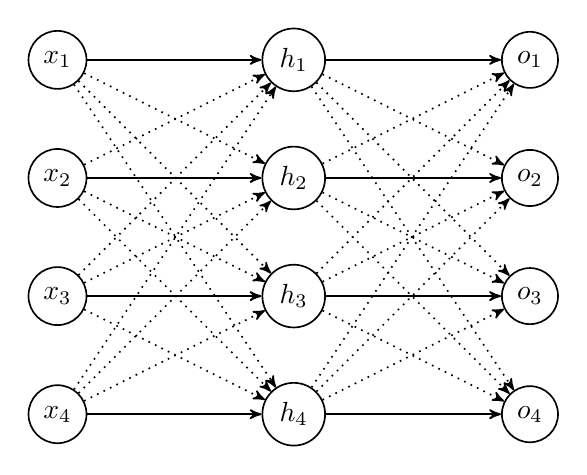
\begin{tikzpicture}[->, >=stealth', auto, semithick, node distance=3cm]
        \tikzstyle{every state}=[fill=white,draw=black,thick,text=black,scale=1]
        \node[draw, circle]    (x1) at (0,0)        {$x_1$};
        \node[draw, circle]    (x2) at (0,-1.5)     {$x_2$};
        \node[draw, circle]    (x3) at (0,-3)       {$x_3$};
        \node[draw, circle]    (x4) at (0,-4.5)     {$x_4$};
        \node[draw, circle]    (h1) at (3,0)        {$h_1$};
        \node[draw, circle]    (h2) at (3,-1.5)     {$h_2$};
        \node[draw, circle]    (h3) at (3,-3)       {$h_3$};
        \node[draw, circle]    (h4) at (3,-4.5)     {$h_4$};
        \node[draw, circle]    (o1) at (6,0)        {$o_1$};
        \node[draw, circle]    (o2) at (6,-1.5)     {$o_2$};
        \node[draw, circle]    (o3) at (6,-3)       {$o_3$};
        \node[draw, circle]    (o4) at (6,-4.5)     {$o_4$};
        \begin{scope}[on background layer]
        \end{scope}
        \path
        (x1) edge[]	node{}	        (h1)
        (x1) edge[dotted]	node{}	(h2)
        (x1) edge[dotted]	node{}	(h3)
        (x1) edge[dotted]	node{}	(h4)
        (x2) edge[dotted]	node{}	(h1)
        (x2) edge[]	node{}	        (h2)
        (x2) edge[dotted]	node{}	(h3)
        (x2) edge[dotted]	node{}	(h4)
        (x3) edge[dotted]	node{}	(h1)
        (x3) edge[dotted]	node{}	(h2)
        (x3) edge[]	node{}	        (h3)
        (x3) edge[dotted]	node{}	(h4)
        (x4) edge[dotted]	node{}	(h1)
        (x4) edge[dotted]	node{}	(h2)
        (x4) edge[dotted]	node{}	(h3)
        (x4) edge[]	node{}	        (h4)
        (h1) edge[]	node{}	        (o1)
        (h1) edge[dotted]	node{}	(o2)
        (h1) edge[dotted]	node{}	(o3)
        (h1) edge[dotted]	node{}	(o4)
        (h2) edge[dotted]	node{}	(o1)
        (h2) edge[]	node{}	        (o2)
        (h2) edge[dotted]	node{}	(o3)
        (h2) edge[dotted]	node{}	(o4)
        (h3) edge[dotted]	node{}	(o1)
        (h3) edge[dotted]	node{}	(o2)
        (h3) edge[]	node{}	        (o3)
        (h3) edge[dotted]	node{}	(o4)
        (h4) edge[dotted]	node{}	(o1)
        (h4) edge[dotted]	node{}	(o2)
        (h4) edge[dotted]	node{}	(o3)
        (h4) edge[]	node{}	        (o4);
        \end{tikzpicture}
        \caption{An MLP with a hidden layer of 4 hidden units.}
      \end{figure}
    \subsection*{Activation Functions}
    \subsubsection*{ReLU Function}
    The most popular choice, due to both simplicity of implementation and its good performance on a variety of predictive tasks, is the rectified linear unit (ReLU) 
    ReLU provides a very simple nonlinear transformation. Given an element $x$, the function is defined as the maximum of that element and 0:
    \begin{equation*}
        \begin{aligned}
            ReLU(x) = \max(x,0)
        \end{aligned}
    \end{equation*}
    When the input is negative, the derivative of the ReLU function is 0, and when the input is positive, the derivative of the ReLU function is 1. Note that the ReLU 
    function is not differentiable when the input takes value precisely equal to 0. In these cases, we default to the left-hand-side derivative and say that the derivative
    is 0 when the input is 0.
    \subsubsection*{Sigmoid Function}
    \begin{equation*}
        \begin{aligned}
            sigmoid(x) = \frac{1}{1+\exp(-x)}
        \end{aligned}
    \end{equation*}
    \subsubsection*{Tanh Function}
    \begin{equation*}
        \begin{aligned}
            tanh(x) = \frac{1-\exp(-2x)}{1+\exp(-2x)}
        \end{aligned}
    \end{equation*}
    
    \subsection*{Forward and Backward Propagation, Computational Graphs}
        \subsubsection*{Forward Propagation}
            Forward propagation (or forward pass) refers to the calculation and storage of intermediate variables (including outputs) for a neural network in order from 
            the input layer to the output layer. 
        \subsubsection*{Backward Propagation}



    \subsection*{Numerical Stability and Initialization}
    \subsubsection*{Vanishing and Exploding Gradients}
    
    \subsubsection*{Parameter Initialization}
    One way of addressing—or at least mitigating—the issues raised above is through careful initialization. As we will see later, additional care during optimization and 
    suitable regularization can further enhance stability.

    \subsubsection*{Default Initialization}
    In the previous sections, we used a normal distribution to initialize the values of our weights. If we do not specify the initialization method, the framework will 
    use a default random initialization method, which often works well in practice for moderate problem sizes.

    \subsection*{Generalization in Deep Learning}
    The TL;DR of the present moment is that the theory of deep learning has produced promising lines of attack and scattered fascinating results, but still appears far 
    from a comprehensive account of both (i) why we are able to optimize neural networks and (ii) how models learned by gradient descent manage to generalize so well, 
    even on high-dimensional tasks. However, in practice, (i) is seldom a problem (we can always find parameters that will fit all of our training data) and thus understanding 
    generalization is far the bigger problem. On the other hand, even absent the comfort of a coherent scientific theory, practitioners have developed a large collection 
    of techniques that may help you to produce models that generalize well in practice. While no pithy summary can possibly do justice to the vast topic of generalization 
    in deep learning, and while the overall state of research is far from resolved, we hope, in this section, to present a broad overview of the state of research and practice.
    
    \subsection*{Dropout}
    
    \section{Builder's Guide}

    \section{Convolutional Neural Networks}
    Image data is represented as a two-dimensional grid of pixels, be it monochromatic or in color. Accordingly each pixel corresponds to one or multiple numerical values
    respectively. So far we ignored this rich structure and treated them as vectors of numbers by flattening the images, irrespective of the spatial relation between pixels.
    This deeply unsatisfying approach was necessary in order to feed the resulting one-dimensional vectors through a fully connected MLP.

    Because these networks are invariant to the order of the features, we could get similar results regardless of whether we preserve an order corresponding to the spatial 
    structure of the pixels or if we permute the columns of our design matrix before fitting the MLP’s parameters. Preferably, we would leverage our prior knowledge that 
    nearby pixels are typically related to each other, to build efficient models for learning from image data.
    \subsection*{From Fully Connected Layers to Convolutions}

    \section{Modern Convolutional Neural Networks}

    \section{Recurrent Neural Networks}

    \section{Modern Recurrent Neural Networks}

    \section{Attention Mechanisms and Transformers}
    Denote by $\mathcal{D} \stackrel{\mathrm{def}}{=} \{(\mathbf{k}_1, \mathbf{v}_1), \ldots (\mathbf{k}_m, \mathbf{v}_m)\}$ a database of $m$ tuples of \emph{keys} and \emph{values}. 
    Moreover, denote by $\mathbf{q}$ a \emph{query}. Then we can define the \emph{attention} over $\mathcal{D}$
    \begin{equation*}
        \begin{aligned}
            \mathrm{Attention}(\mathbf{q}, \mathcal{D}) \stackrel{\mathrm{def}}{=} \sum_{i=1}^m \alpha(\mathbf{q}, \mathbf{k}_i) \mathbf{v}_i,
        \end{aligned}
    \end{equation*}
    where $\alpha(\mathbf{q}, \mathbf{k}_i) \in \mathbb{R}$ are scalar attention weights. The operation itself is typically referred to as \emph{attention pooling}.  
    The name attention derives from the fact that the operation pays particular attention to the terms for which the weight $\alpha$ is significant (i.e., large). 
    As such, the attention over $\mathcal{D}$ generates a linear combination of values contained in the database. This opens a number of special cases, namely
    \begin{itemize}
        \item The weights $\alpha(\mathbf{q}, \mathbf{k}_i)$ are nonnegative. In this case the output of the attention mechanism is contained in the convex cone spanned by the values $\mathbf{v}_i$.
        \item The weights $\alpha(\mathbf{q}, \mathbf{k}_i)$ form a convex combination, i.e., $\sum_i \alpha(\mathbf{q}, \mathbf{k}_i) = 1$ and $\alpha(\mathbf{q}, \mathbf{k}_i) \geq 0$ for all $i$. 
        This is the most common setting in deep learning.
        \item Exactly one of the weights $\alpha(\mathbf{q}, \mathbf{k}_i)$ is $1$, while all others are $0$. This is akin to a traditional database query.
        \item All weights are equal, i.e., $\alpha(\mathbf{q}, \mathbf{k}_i) = \frac{1}{m}$ for all $i$. This amounts to averaging across the entire database, also called average pooling in deep learning.
    \end{itemize}

    \newpage
    \subsection*{Miscellaneous}
    Variational autoencoders
    Standard distribution
    non-standard distribution gaussian
    What is the difference between 
    why do we initialize parameters with gaussian noise
    How are activation fuctions used
\end{document}